\documentclass[float=false, crop=false]{standalone}
\usepackage[subpreambles=false]{standalone}
\usepackage{import}

\usepackage{subfiles}
\usepackage[backend=biber,style=numeric,sorting=none]{biblatex}
\usepackage[pdfborder={0 0 0}]{hyperref}   
\usepackage[margin=25mm]{geometry} 
\usepackage{graphicx}  
\usepackage[utf8]{inputenc}
\usepackage{textcomp}
\usepackage{import}
\usepackage[font=small,labelfont=bf]{caption}

\usepackage{stmaryrd}
\usepackage{verbatim}
\usepackage{amsmath}
\usepackage{amsfonts}
\usepackage{amssymb}
\usepackage{amsthm}
\usepackage{sansmath}
\usepackage{mathtools}

\usepackage{pgfgantt}
\usepackage{graphicx}
\usepackage{xcolor}

\ganttset{group/.append style={orange},
          milestone/.append style={red},
          progress label node anchor/.append style={text=red}}

\usepackage{color}

\newlength\gwidth
\newlength\gheight
\setlength{\gwidth}{\textwidth}
\setlength{\gwidth}{\textheight}


\usepackage[capitalize, nameinlink]{cleveref}
\crefdefaultlabelformat{#2\textbf{#1}#3}

\crefname{figure}{\textbf{Figure}}{\textbf{Figures}}
\crefname{table}{\textbf{Table}}{\textbf{Tables}}
\crefname{appendix}{\textbf{Appendix}}{\textbf{Appendices}}

\definecolor{pblue}{rgb}{0.13,0.13,1}
\definecolor{pgreen}{rgb}{0,0.5,0}
\definecolor{pred}{rgb}{0.9,0,0}
\definecolor{pgrey}{rgb}{0.46,0.45,0.48}

\usepackage{listings}
\lstnewenvironment{JavaLst}
{\lstset{language=Java,
  showspaces=false,
  showtabs=false,
  breaklines=true,
  showstringspaces=false,
  breakatwhitespace=true,
  commentstyle=\color{pgreen},
  keywordstyle=\color{pblue},
  stringstyle=\color{pred},
  basicstyle=\ttfamily,
  moredelim=[il][\textcolor{pgrey}]{$$},
  moredelim=[is][\textcolor{pgrey}]{\%\%}{\%\%},
  escapeinside={&}{&}
}}{}

\lstnewenvironment{HaskellLst}
{\lstset{
  frame=none,
  xleftmargin=2pt,
  stepnumber=1,
  numbersep=5pt,
  numberstyle=\ttfamily\tiny\color[gray]{0.3},
  belowcaptionskip=\bigskipamount,
  commentstyle=\color{pgreen},
  keywordstyle=\color{pblue},
  stringstyle=\color{pred},
  basicstyle=\ttfamily,
  captionpos=b,
  escapeinside={*'}{'*},
  language=haskell,
  tabsize=2,
  emphstyle={\bf},
  commentstyle=\it,
  showspaces=false,
  columns=flexible,
  showstringspaces=false,
  morecomment=[l]\%,
}} {}

\lstnewenvironment{JVMLst}
{\lstset{
  frame=none,
  numbers=none,
  xleftmargin=2pt,
  language=JVMIS,
  emphstyle={\bf},
  stringstyle=\mdseries\rmfamily,
  commentstyle=\color{pgreen},
  stringstyle=\color{pred},
  keywordstyle=\color{black},
  basicstyle=\ttfamily,
  basicstyle=\small\sffamily
}} {}

\usepackage{tikz}
\usetikzlibrary{positioning}

\tikzset{
  treenode/.style = {shape=rectangle, rounded corners,
                     draw, align=center,
                     top color=white, bottom color=blue!20},
  root/.style     = {treenode, font=\ttfamily\Large},
  env/.style      = {treenode, font=\ttfamily\normalsize},
  dummy/.style    = {circle,draw}
}

\newcommand{\tlang}{\bigstar}
\newcommand{\thunk}[1]{\lceil #1 \rceil}
\newcommand{\unwrap}[1]{\lfloor #1 \rfloor}
\newcommand{\tcbn}{\rightarrow_N}
\newcommand{\tcbv}{\rightarrow_V}
\newcommand{\tccbv}{\rightarrow_V^*}
\newcommand{\tthunk}{\rightarrow_\tlang}
\newcommand{\tlthunk}{\rightsquigarrow_\tlang}

\begin{document}

The compiler implementation was split up into work packages.
A work package involved the implementation of one, 
or only a part of a stage, depending on an estimation of how long 
each stage would take to implement.


% Work packages were then formed from these five stages --
% some weeks contained a whole compiler stage, while other work packages contained
% only part of a compiler stage.

% \section{Overview}
% A functional compiler is usually though of as a five stage pipeline consisting of:

% \begin{enumerate}
%   \item Lexing and Parsing.
%   \item Desugaring.
%   \item Type Checking.
%   \item Optimisation.
%   \item Code Generation.
% \end{enumerate}
% This is how I will split up the implementation of the compiler.

% \section{Lexing and Parsing}

% Parsing and lexing of programming is a well research problem with 
% powerful tools that can be used to implemented a lexer and parser, so
% will details will be given of this stage when compared to others.


% The Haskell 98 report \cite[2.]{haskell98-spec} provides a full specification
% of lexing rules, I implemented a subset of these rules using 
% Alex\cite{alex-lib}. This transform will go from a input text to a set
% of lexical tokens. These tokens are expressed using the datatype
% \texttt{LToken}.

% The Haskell 98 report \cite[3.]{haskell98-spec} provides a full specification
% of parsing rules, which again I implemented a subset of, this time using
% the parsing generator Happy\cite{happy-lib}.


% \section{New notes}

% Maybe add a code diagram UML like or something...
% Maybe outline in slightly more details how pipeline maps to code.


\section{Work division}

A waterfall model was used to develop the compiler, since I was the only 
person working on the compiler and requirements were clear at the start and unlikely to change. 
This resulted in a linear ordering to work packages being completed. 
\cref{figure:ganttchar} shows how the project progressed. The first
few weeks matched up to the proposed timetable given the project proposal, however implementing
the type inference (TI) was quicker than expected meaning that the only slack given (over the Christmas
holidays) was not needed and I started work on future work packages. 
The slack time was very generous, if 
no slack time was allocated to this project it would have been delivered only one week ahead of schedule. 
The code generation section took a little
longer than usual. This is due to in part to implementing the
translation from the core calculus to JVM bytecode. To fully understand
the problem I formalised this translation. This 
made the code generation work packages longer than expected. It also
took longer than expected to implement the bytecode translation due
to me not fully understanding the semantics of JVM bytecode. I 
needed to rewrite large parts of the code generation stage after 
understanding the bytecode semantics. In hindsight a better understanding
of the JVM bytecode specification would have saved time
overall. Next time I would allocate extra time, before writing any code, to 
understanding the JVM bytecode specification in more detail.

\subimport{workStages/}{workStageGantt.tex}

% \section{Lexing and Parsing}

% \begin{itemize}
%   \item Maybe show a small subset of the grammar and expression and how
%     that can be implemented in Alex and Happy. 

%   \item Talk about how it can be implemented as an LR(0) parser.
% \end{itemize}

% \section{Desugaring}

% \begin{itemize}
%   \item Talk about kind inference, this can be related closely to 
%     TI, so used a very similar method as used in TI.

%   \item Maybe talk about simple different between desugared before and after.

%   \item Talk about build-in datatypes being added to the desugaring.

% \end{itemize}

\section{Lexing, Parsing and Desugaring}

The Lexer was simple to implement with the help of Alex \cite{alex-lib}.
The Haskell grammar accepted by JVHC was possible to express using an
LR(0) grammar and therefore could be implemented in Happy \cite{happy-lib}
without much trouble. The desugaring stage involved kind inference
mentioned in the preparation section (this was very similar to type inference).
The desugaring also involved a set of simple syntax tree transformations, 
which need not be explained here.

\section{Type Inference}

The type inference stage in JVHC was heavily influenced by a paper
called `Typing Haskell in Haskell' \cite{thih-paper}. This paper laid 
out an implementation in Haskell of how to run type inference
over a whole Haskell program and find the type of each definition.
I will therefore not go into detail about the implementation of the 
type inference itself. I will however talk about moving from a Haskell
syntax tree to a valid system F like core language.
This process was interleaved with the type inference algorithm.
That meant the result of running type inference gave a type for each
top level function, and also a new datatype called \texttt{CoreExpr}

The full CoreExpr datatype is listed in \cref{code:CoreExpr}. 
All the types in this datatype
are directly from System F, apart from case. The \verb|Case|
construct allows pattern matching different constructors of an ADT 
and conditionally executing different branches of the \verb|Case| expression.
The datatype is parameterised on \texttt{b}, this is a binder type which 
stores only the variable name and type.

\begin{figure}
  \centering
  \begin{lstlisting}[language = Haskell, escapechar = !]
        data Expr b
          = Var  Id
          | Lit  Literal
          | App  (Expr b)     (Arg  b)!
          \tikz[remember picture] \node [] (arg) {};
          !
          |!
           \tikz[remember picture] \node [] (lam) {};
         !Lam  b            (Expr b)
          | Let  (ExprDef b)  (Expr b)
          | Case (Expr b)     Type     [Alt b]!
          \tikz[remember picture] \node [] (alts) {};
          !
          |!
          \tikz[remember picture] \node [] (type) {};
          !Type Type

        data ExprDef b = ExprDef b (Expr b)
  \end{lstlisting}
  \begin{tikzpicture}[remember picture, overlay,
    every edge/.append style = { ->, thick, >=stealth,
                                   dashed, line width = 0.5pt },
    every node/.append style = { align = center, minimum height = 10pt,
                                 font = \bfseries, fill={rgb:black,1;white,20}},
                  text width = 2.5cm ]
  \node [left = 0.5 cm of lam,text width = 2.2cm]
                             (Lam) {Could be $\Lambda$ or $\lambda$.};
  \node [right = 0.5 cm of arg,text width = 2.2cm]
                             (Arg) {Could be a \texttt{Expr} or a \texttt{Type}.};
  \node [right = 0.5 cm of alts,text width = 2.2cm]
                             (Alts) {List of possible branches.};
  \node [left = 0.5 cm of type,text width = 2.2cm]
                             (Type) {Types erased for code gen.};
  \draw (Lam.east)  + (0, 0) coordinate(x1) edge (lam.east|-x1);
  \draw (Arg.west)  + (0, 0) coordinate(x1) edge (arg.west|-x1);
  \draw (Alts.west) + (0, 0) coordinate(x1) edge (alts.west|-x1);
  \draw (Type.east) + (0, 0) coordinate(x1) edge (type.east|-x1);
\end{tikzpicture} 
  \caption[Listing of \texttt{CoreExpr} datatype]{Listing of \texttt{CoreExpr} datatype. The \texttt{Type} type represents any possible type valid
    in Haskell, this is the same type datatype as in the 
    type inference section above.}
  \label{code:CoreExpr}
\end{figure}
The resulting code returned from the mixed type inference and syntax transform stage was not quite
valid \texttt{CoreExpr}. To convert this resulting syntax tree to valid System F, type information
needs to be added explicitly (in a ``fix-up'' stage), this meant adding both type applications and $\Lambda$ (type abstractions)
to the syntax. To add these constructs a lookup table was also returned to the type inference stages, 
which contained the type of every sub-expression. This was used to insert type applications and
$\Lambda$ in the correct places in the syntax tree making the resulting syntax tree valid again. Since each type in Haskell \verb|a -> [a]| has an implicit
$\forall$, and so can be written as \verb|forall a.a -> [a]|, the $\Lambda$
must always be at the very beginning of an expression if there are any
$\forall$ bound variables in the type. Then every time there is an application $e_1 e_2$, 
some number of type application must be inserted matching the 
$\Lambda$s in $e_1$ to the expression making the new expression
$e_1 \tau_1 \dots \tau_n e_2$.
The reason that the type inference includes a syntax transformation is twofold, first it 
means only a single walk of the tree is required when generating the \verb|CoreExpr| datatype. Second
the type variables generated in type inference are used as temporary variables in the 
resulting \verb|CoreExpr| datatype. 
Once the constraints generated in type inference have been solved the constraint variables are replaced with the correct types in the outputted \verb|CoreExpr| syntax tree.
The ``fix-up'' phase is necessary after type inference as the \verb|CoreExpr| can only be corrected to
valid System F once a full type of every expression is known, which is only known after type inference. 

% \begin{itemize}
%   \item Talk about paper.

%   \item Talk about understanding the paper

%   \item Talk about modification I made to remove type classes.

%   \item Talk about going to the broken core output
%     from TI, to valid system F in the form with all $\Lambda$ at the 
%     start of the expression and with the correct inserted types.

%   \item Talk about build in functions being added to the TI.
% \end{itemize}

\section{Inlining}

% \begin{itemize}
%   \item Talk about general principle a bit.

%   \item Talk about the inline monad and the \texttt{inline} function
%     and the \texttt{rename} function and monad.

%   \item Talk about when to inline, don't inline recursive functions.
%     Be careful inlining \texttt{id x = id x}.

%   \item Talk about inline metric to decide whether a function should be inlined.
% \end{itemize}

Function inlining is based on the idea that it 
would be better to inline some functions, so as
to remove the need for the function call to happen. 
Also if a function has been inlined, this might allow further
optimisations to occur, such as constant folding.

Constant folding is replacing a branch instruction
(in Haskell a \verb|case| expression), where the outcome is 
known at compile time with the code for the taken branch only.

I will first explain constant folding in more detail since
it is a simpler concept.
Given an expression 
\begin{HaskellLst}
case 2 of 
  1 -> e
  2 -> e'
\end{HaskellLst}
Using constant folding this expression would be reduced to
\begin{HaskellLst}
e'
\end{HaskellLst}
Function inlining is a more interesting problem. The technique I used
was heavily influenced by the paper \cite{ghc-inliner}, which 
revolves around deciding when to inline the expression:
\begin{HaskellLst}
let x = e' in e
\end{HaskellLst}
where \verb|e| may contain free (unbound) occurrences of \verb|x|.
Lambda functions can be $\beta$-reduced ($(\lambda x.e) e' \rightarrow_\beta e[e'/x] $) 
to a \verb|let| construct, meaning that
\begin{HaskellLst}
(\x -> e) e'
\end{HaskellLst}
goes to
\begin{HaskellLst}
let x = e' in e 
\end{HaskellLst}
When inlining a function name the expression, that represents 
that function body, must first be $\alpha$-renamed 
using fresh variables (or type variables) which don't exist 
anywhere in the program. This is done by using a ASCII character 
which is not allowed in either function or type name, \texttt{*}
was used.
\verb|CoreExpr| also contains $\Lambda$ abstractions of type
variables. When inlining $\beta$-reduction is also applied to types using
the rule:
\[ (\Lambda t.e) t' \rightarrow_\beta e[t'/t] \]
where $e[a/x]$ means substitute all free occurrences of $x$ in $e$
with $a$.

When to inline the \verb|let| construct is a very hard
question to answer. We should make sure of two things: one, the 
inliner must terminate, therefore we cannot inline recursive 
functions forever; and two, we wish inlined code to 
perform better (in whatever metric we use) when compared to the original
code.
First I will consider the termination of the inliner, this can be assured by 
not inlining any recursive functions.
The second problem contains lots of subtlety. 
The performance metric considered here is a smaller runtime. Two things must
be computed to decide if inlining is a good idea, 
the cost of computing \verb|e'| and the number of times
\verb|x| appears in \verb|e|. We want the cost of computing
\verb|e'| to be small and the number of times \verb|x| appears
in \verb|e| to also be small. I came up with a very simple
metric:
\begin{itemize}
  \item I assumed the cost of \verb|e'| to be constant.
    It is not possible in general to know the cost at compile time, 
    therefore heuristics must be used. 
    For example if the expression \verb|e'| contained any 
    recursive functions then it may have a higher cost to 
    compute \verb|e'|, than a function without any recursive function 
    calls inside.

  \item The number of times \verb|x| is free in \verb|e'|
    easily can be be computed, then any time that
    there are four or more free occurrences, don't inline.
    If there are fewer than four free occurrences then inline.
\end{itemize}

A function is syntactically recursive if there is mention of the
function name inside the function body. This is an over-approximation
since it may be the case that the function never recurses, however
that cannot be known at compile time, hence an approximation is
used instead.
When counting the number of times a variable is free in an expression, 
it suffices to count each time the variable name exists in the syntax tree, 
until it is rebound in a $\lambda$-function, at which point the current count 
is returned for that branch in the syntax tree. The \verb|Case| expression can have multiple
branches in the tree each of which may have a different count
for the occurrence of a variable name, the maximum occurrence over all these
branches is returned.

\section{Code Generation}

% \begin{itemize}
%   \item Talk about how each part of the syntax tree was converted from 
%     CoreExpr to classes.

%   \item Link back to original proposal before coding about how to implement
%     everything.

%   \item Talk about verifiable bytecode.

%   \item 
% \end{itemize}

During the preparation phase I created a document describing the 
translation from the CoreExpr data-type to JVM bytecode.
After considering the input data \texttt{CoreExpr}, next I considered what the result of each element 
of the datatype would map to. I have shown the mapping from the \texttt{CoreExpr} datatype to
Java code for the readers convenience, however in the compiler the conversion was to JVM bytecode.
This compiler must emulate a computation that can be carried out at a later date. This can be implemented
using thunks.
A thunk can be thought of as a nullary function (one which takes no arguments) and when required will 
perform a computation. If we have an expression $e$ we can wrap it inside a thunk $\lambda (). e$  then 
only when we apply $()$ to this thunk does the computation take place, this allows the
simulation of call-by-name semantics
when the program is being run with call-by-value operation semantics. 
In JVHC this will be implemented by creating a class
which implements a method \verb|force|, which will be called by \verb|get| in the default
implementation of a thunk.
\begin{JavaLst}
public abstract class Thunk<T> implements Supplier<T> {
    private T value;
    protected abstract T force();
    @Override
    public T get() {
        if ( value == null ) {
            return value = force();
        }
        return value;
    }
}
\end{JavaLst}
The important part of this implementation is that once \verb|force| has been called once
the value will be cached inside this class and future calls to \verb|get| will result
in the cached value being returned. The thunk class will implement the supplier interface:
\begin{JavaLst}
public interface Supplier<T> { T get(); }
\end{JavaLst}
in the hope of better integration with existing Java 8 functional interfaces.
Functions will implement the Function interface
\begin{JavaLst}
public interface Function<T, R> { R apply(T t); }
\end{JavaLst}
When first implementing code generation, there were bugs in the implementation
where the mapping between \texttt{CoreExpr} and the lazy language implemented
via the use of thunks. Due to the bugs in the first attempt to implement the 
translation I decided to formalise the translation.
The result was a mathematical framework for expressions defining both 
a core calculus which defines how Haskell could theoretically execute and 
core calculus$_\bigstar$ which is similar to how expressions will
execute on the JVM. This is included in \cref{appendix:thunkProof}. 
The notation $\thunk{e}$ means, the value $e$ is wrapped in a thunk. Then
$\unwrap{t}$ means reduce the expression to a value from the thunk $t$. 
This would directly map to calling \texttt{get} when implemented in 
JVM bytecode. The translation relation $\tlthunk$ from core 
calculus to core calculus$_\bigstar$ is defined as:
\begin{align*}
  &\frac{}{c \tlthunk \thunk{c}}\\ \\
  &\frac{}{x \tlthunk \thunk{x}}\\ \\
  &\frac{e \tlthunk e_\tlang}
     {\lambda x . e \tlthunk \thunk{\lambda x_\tlang.\unwrap{e_\tlang}}}\\ \\
  &\frac{e  \tlthunk e_\tlang \quad e' \tlthunk e'_\tlang}
  {e e' \tlthunk \thunk{\unwrap{e_\tlang} e'_\tlang}}\\ \\
  &\dfrac{e_1  \tlthunk e_{1_\tlang} \quad \dots \quad e_n \tlthunk e_{n_\tlang} \quad e' \tlthunk e_\tlang}
  {\splitdfrac{\mathtt{let}\ (x_1\ \mathtt{=}\ e_1,\dotsc, x_n\ \mathtt{=}\ e_n)\ \mathtt{in}\ e \tlthunk}
    {\thunk{\mathtt{let}\ 
        (x_1\ \mathtt{=}\ e_{1_\tlang},\dotsc, x_n\ \mathtt{=}\ e_{n_\tlang}) \ \mathtt{in}\ \unwrap{e_\tlang}}}}\\ \\
  &\dfrac{e_1  \tlthunk e_{1_\tlang} \quad \dots \quad e_n \tlthunk e_{n_\tlang} \quad e' \tlthunk e'_\tlang}
  {\splitdfrac{\mathtt{case}\ e\ \mathtt{of}\ b_1 \rightarrow e_1; \dots; b_n \rightarrow e_n \tlthunk}
  {\thunk{\mathtt{case}\ \unwrap{e_\tlang}\ \mathtt{of}\ b_1 \rightarrow \unwrap{e_{1_\tlang}}; 
      \dots; b_n \rightarrow \unwrap{e_{n_\tlang}}}}}
\end{align*}
From this, \cref{appendix:thunkProof} proves
that the call-by-name transition relation that Haskell should implement
as defined in the Haskell 98 report will map directly to a 
finite number of call-by-value transition relation steps, 
which execute in a similar way to the JVM.

\subsection{Variable scope}
There are two places that variables can be introduced.
\begin{itemize}
  \item In $\lambda$ functions, each closure will contain a reference
    to thunk object that is passed into the closure, this argument
    can then been queried later.
  \item Top level \texttt{let} binding
    which can contain many references to many variables. These
    will be in the form of thunks defining all top level functions.
\end{itemize}
The following code example would be laid out in a scope hierarchy as in 
\cref{figure:scope_map}.
\begin{HaskellLst}
id x  = x
three y = case y of
  (l:ls) -> 0
\end{HaskellLst}
\begin{figure}
  \centering
  \resizebox{\columnwidth}{!}{
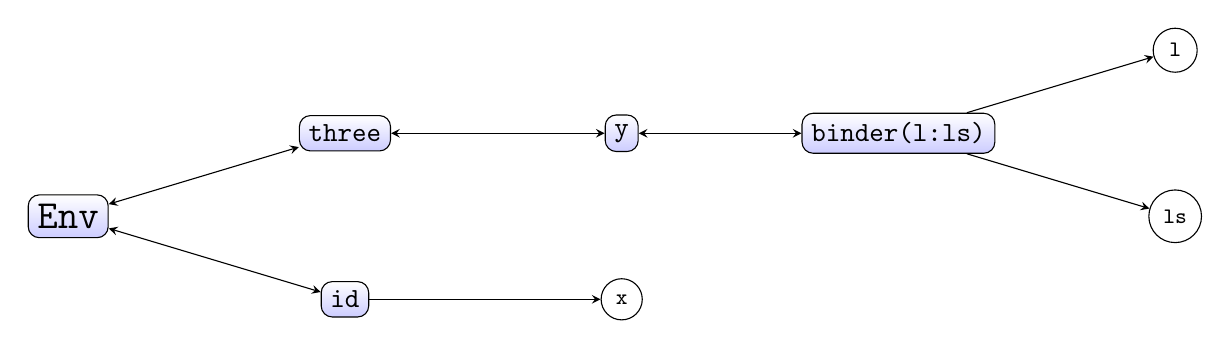
\begin{tikzpicture}
  [
    grow                    = right,
    sibling distance        = 6em,
    level distance          = 10em,
    edge from parent/.style = {draw, -latex, >=stealth},
    every node/.style       = {font=\footnotesize},
    sloped
  ]
  \node [root] {Env}
    child { node [env] {id}
         child { node [dummy] {\texttt{x}}
              edge from parent [->] node [below] {} } 
         edge from parent [<->] node [below] {} }
    child { node [env] {three}
         child { node [env] {\texttt{y}}
             child { node [env] {\texttt{binder(l:ls)}}
               child { node [dummy] {\texttt{ls}}
                         edge from parent [->] node [above] {}  }
               child { node [dummy] {\texttt{l}}
                         edge from parent [->] node [below] {} }
             edge from parent [<->] node [below] {} }
         edge from parent [<->] node [below] {} } 
    edge from parent [<->] node [below] {} };
\end{tikzpicture}
  }
\caption[Scope and class hierarchy]{Scope and class hierarchy, blue boxes are classes, and white circles are
references to variables. Arrows signify a reference to the object
being pointed to in the object from which the arrow stems.}
\label{figure:scope_map}
\end{figure}
The top level functions of the program will be stored in an \verb|Env| class,
then each possibly mutually recursive function will have a reference 
to every other function, via the \verb|Env| class.

\subsection{CoreExpr Constructs}

When generating bytecode each construct in the \verb|CoreExpr| type is 
considered in turn. For each construct considered the result will be
a list of bytecodes which will be consumed by the parent of this node.
It is also possible that a separate \verb|.class| file will
be created (in the case of a $\lambda$-function say). Then the parent
of a \verb|CoreExpr| tree will be the top level scope class 
called \verb|Env|. This will contain references to all top level functions
and a \verb|main| method. The main method allows this program
to be run as a standalone program. The \verb|Env| class
can also be accessed from other JVM compatible programming
languages. The \verb|Env| class will expose the top level functions
defined in the source file. I will now go over 
each of the 6 constructs in turn explaining how they are 
translated into JVM bytecode:

\begin{itemize}
\item The \texttt{Lit} construct will be represented as either a
\texttt{CharThunk} or an \texttt{IntThunk} containing the value
of the literal.

\item The \texttt{Var} construct will either be a built-in function
(in which case it will be a thunk that when evaluated will return the built in
value), or a user defined function/datatype.

\item The \verb|Lam b e| construct will generate the following
code in a separate class file:
\begin{JavaLst}
public class &\textit{NAME}& implements Function {
  &\textit{ty}&(&\textit{t}&) arg;
  &\textit{Parent}& p;
  &\textit{NAME}& (&\textit{Parent}& p) {
    this.p = p
  }

  protected &\textit{ty}&(&\textit{e}&) (&\textit{ty}&(&\textit{b}&) arg) {
    this.arg = arg
    return &$\llbracket \textit{e} \mkern2mu  \rrbracket$&.get();
  }
}
\end{JavaLst}
The {\ttfamily \textit{NAME}} will be the unique name of the function.
The {\ttfamily \textit{ty}} will return the Java type {\ttfamily \textit{t}} 
of either the binder \texttt{b} or the expression in the lambda \texttt{e}, and 
{\ttfamily $\llbracket \textit{e}  \mkern2mu \rrbracket$} is a sequence
of expression produced by converting {\ttfamily\texttt{e}} to a JVM bytecode.
The code snippet returned will create a function object for the function
referenced in the \verb|CoreExpr| datatype and then wrap it inside a thunk.
This is the Java implementation of translation relation $\tlthunk$ above.
\begin{JavaLst}
new ObjThunk(new &\textit{Name}&(&\textit{Parent}&));
\end{JavaLst}

\item The \verb|App| mapping first creates a class which represents the thunk for \verb|App e1 e2|, 

\begin{JavaLst}
public class &\textit{AppName}& implements Thunk {
  &\textit{Parent}& p;
  &\textit{NAME}& (&\textit{Parent}& p) {
    this.p = p
  }

  public force() {
    return (Supplier)(&$\llbracket \mkern1mu \textit{e}_1 \rrbracket$&.get()).apply(&$\llbracket \mkern1mu \textit{e}_2 \rrbracket$&);
  }
}
\end{JavaLst}
Then the returned source code is 
\begin{JavaLst}
new &\textit{AppName}&(&\textit{Parent}&);
\end{JavaLst}

\item \verb|Let| is just mapped to \verb|Lam| and then converted to JVM bytecode in the same
  way that \verb|Lam| is.

\item \verb|Case| is mapped to a sequence of conditions where the case binder is checked against the 
  value being scrutinised. There are examples in 
  \cref{appendix:bytecodetranslationdoc}

\end{itemize}

\subsection{Using Codec-JVM}

The library used to format JVM bytecode was \textit{codec-jvm}. This provides
a simple to use Haskell interface to write JVM bytecode.
The library exposes a type called \verb|Code| which is a monoid. 
In Haskell, a monoid requires two functions to be defined
\verb|mempty| and \verb|<>| (called \verb|mappend|), 
the first returns an empty value and the 
second takes two variables of type \verb|Code| and combines them, returning
a new \verb|Code| variable.
Variables with type \verb|Code| map closely to JVM bytecode instructions.
For example there is a function \verb|new|$_\text{Hask}$ which takes a Java type 
and returns a variable of type \verb|Code|, 
this is very similar to the JVM bytecode instruction
\verb|new|$_\text{JVM}$. The JVM \verb|new|$_\text{JVM}$ instruction creates
an object of the type passed as an operand to this bytecode instruction. 
Then the following Haskell code:
\begin{HaskellLst}
   new             &\textit{ObjType}& 
<> dup             &\textit{ObjType}&
<> invokespecial &\textit{ObjTypeConstructor}&
\end{HaskellLst}
maps directly to
\begin{JVMLst}
new           #2            // class ObjType
dup
invokespecial #3            // Method ObjType."<init>":()V
\end{JVMLst}
The convenient Haskell interface and control flow handling 
are main the features that I used from \textit{codec-jvm}.

\subsection{Generating Correct JVM Bytecode}

When loading \verb|.class| files the JVM will run a verifier (as defined
by the JVM specification \cite[\S 4.10]{jvm-spec8}) on the 
loaded bytecode. The verifier will check to make sure that:
\begin{itemize}
  \item There are no operand stack overflows or underflows.

  \item All local variables uses and stores are valid.

  \item The arguments to all the JVM instructions are of valid types.
\end{itemize}
These verification conditions helped to debug the outputted code. 
When I started out generating bytecode I was generating code
which didn't conform to all of these verification conditions.
\verb|CoreExpr| constructs each generated a small piece of
code $C$, this meant it was hard at first to make sure
that no $C$ would add or remove the wrong number of operands. It was very
helpful that when the \verb|.class| file was loaded, that the verifier
would give immediate feedback. The verifier also checked that
after each branch the type of each element on the stack
was the same, this again was very helpful when debugging \verb|case|
statements. This meant I could be sure that each branch of a case statement
would return a stack with each element being the same type (or sharing a 
common parent type).


\section{Runtime Library}

There is a small runtime library included with JVHC, this library is implemented in Java code.
This allowed for arbitrary side effect free Java code to be invoked by Haskell code. 
The JVHC compiler must also be made aware of the type and Java name of each of the functions exposed from 
the Java world. This means exposing a new function to JVHC will
require the source of the compiler to be edited. 
To improve the compiler a configuration file could be used, or even better
a keyword in the source to expose new functions to Haskell.
The runtime is bundled in the package \verb|BuiltIn| and includes, for example,
a function \texttt{add} to sum two integers.

\subsection{I/O Monad}

Haskell, as mentioned previously, is a pure language without side effects. If Haskell
is to allow I/O or any possible side effect, then this can be implemented using an I/O
monad abstraction. The I/O monad represents a sequence of instructions that when run will result in 
the sequence operations being executed in the order they were defined in the 
program (not the order they were evaluated, since Haskell is lazy
these two may be different). The I/O monad can only be run by the runtime
of the program. This happens when the I/O monad is returned from the executing 
\verb|main| function at which point the runtime will force evaluation of the 
I/O monad.
The following code will continuously read a value and print out 
twice that value
\begin{HaskellLst}
times2 :: IO Int
times2 = getInt >>= (\i -> putInt (i*2) >> times2)
\end{HaskellLst}
\verb|getInt :: IO Int| creates a monad that when evaluated (by the runtime)
will try to read an integer from stdin.
\verb|>>= :: IO a -> (a -> IO b) -> IO b| (pronounced bind) is used to combine monads.
\verb|>>=| allows access to the value inside the monad (this is 
useful since at the current point of execution, the value 
which will be passed to the function is not yet known). 
Then \verb|>>| is similar to \verb|>>=| but ignoring the result of 
the first monad. The I/O monad is implemented as a Java interface
\begin{JavaLst}
public interface IO<R> { R unsafePerformIO(); }
\end{JavaLst}
Then in the runtime will call \verb|unsafePerformIO| on the return value of the \verb|main|
function.

\section{Open Source contribution}

When using the \textit{codec-jvm} library for code generation I
extended the library adding support for JVM bytecode instructions not already
implemented by the library.
Support was added  for \verb|instanceof|, \verb|dup_x1| and \verb|athrow|. 
I then created a Github pull request and the change was merged 
into the master branch of the library \cite{codec-contrib}.

% \section{Benchmarking}

% \begin{itemize}
%   \item Talk about fully evaluating expression in Haskell, not just
%     weak head normal form.

%   \item Talk about Criterion for simple Haskell benchmark.

%   \item Talk about how the benchmarker was implemented to test
%     multiple run of compiled Haskell program. Could talk
%     about Haskell system programming.
% \end{itemize}

\end{document}
